\documentclass[a4paper]{scrreprt}
\usepackage{fancyhdr}
\pagestyle{fancy}
\usepackage[english]{babel}
\usepackage[utf8]{inputenc}
\usepackage{graphicx}
\usepackage{url}
\usepackage{textcomp}
\usepackage{amsmath}
\usepackage{lastpage}
\usepackage{pgf}
\usepackage{wrapfig}
\usepackage{fancyvrb}

% Create header and footer
\headheight 27pt
\pagestyle{fancyplain}
\lhead{\footnotesize{Object-Oriented Design, IV1350}}
\chead{\footnotesize{Seminar 1 Solution}}
\rhead{}
\lfoot{}
\cfoot{\thepage\ (\pageref{LastPage})}
\rfoot{}

% Create title page
\title{Seminar 1}
\subtitle{Object-Oriented Design, IV1350}
\author{Pontus Söderlund, psoderlu@kth.se}
% \date{\today} Prints today's date
\date{March 30th}

\begin{document}

\maketitle

\tableofcontents %Generates the TOC

\chapter{Introduction}
    % A summary of the seminar task. Also, tell who you worked with when solving the task. 
    The goal of this seminar is to create a domain model (DM) for a retail store
    and a system sequence diagram (SSD) for a sale.

\chapter{Method}
    % Explain how you arrived at the solution presented in chapter \ref{sec:result}.
    % For example, one of the things to explain in the report for seminar one, is
    % how you used a category list and noun identification to find class candidates
    % for the domain model.
    
    \section{Domain Model}
        The process for creating a domain model can be borken down into five the 
        five steps listed bellow.

        \subsection{Identify class candidates}
            The first step is to read the specification and find all the nouns in
            in it. For the requirements in this lab some of the words found are
            listed below.

            \begin{itemize}
                \item Customer
                \item Goods
                \item Cashier
                \item Register
                \item Cash
                \item Change
                \item Program
                \item Reciept
            \end{itemize}

        \subsection{Use a category list}
            The second step is to use a category list to find even more class
            candidates.

            A category list is a tool to help find more class candidates by
            giving examples of categories that things not tought of in the first
            step belongs to. The project requiremients might for  
        
        \subsection{Filter class candidates}
            The next step is to filter out the class candidates that do not
            provide any additional value. It might be that one was too thorugh
            in previous steps or that the same information is in multiple places
            or something similar.
            
            In this case it 

        \subsection{Find attributes}
            After having filtered the class candidates I identified classes that
            were more suitable as attributes to classes. 
            
            Attributes are things that describe a class and not something that's
            part of it. A clear example of an attribute is a customer id since
            it is just an identifier for any given customer. An example of
            something that's not an attribute is a reciept since it can exist
            independently of a transaction.

        \subsection{Add associations}
            The last step is to att associations between the different classes.
            The program I used did not have any way (that I found) to create
            the > (Class 1 Verb > Class 2) notation used in the lectures, I
            decided to use the directional association arrows instead. 

    \section{System Sequence Diagram}
            

\chapter{Result}
    \label{sec:result}
    % This chapter shall contain the solution to the seminar tasks, together with
    % a short explanation. There are more detailed instructions in each
    % assignment.

    % Remember that code extracts and diagrams must be numbered, have caption and
    % be explained in the text, see figures \ref{fig:diag} and \ref{fig:code}

    \begin{figure}[h!]
        \begin{center}
            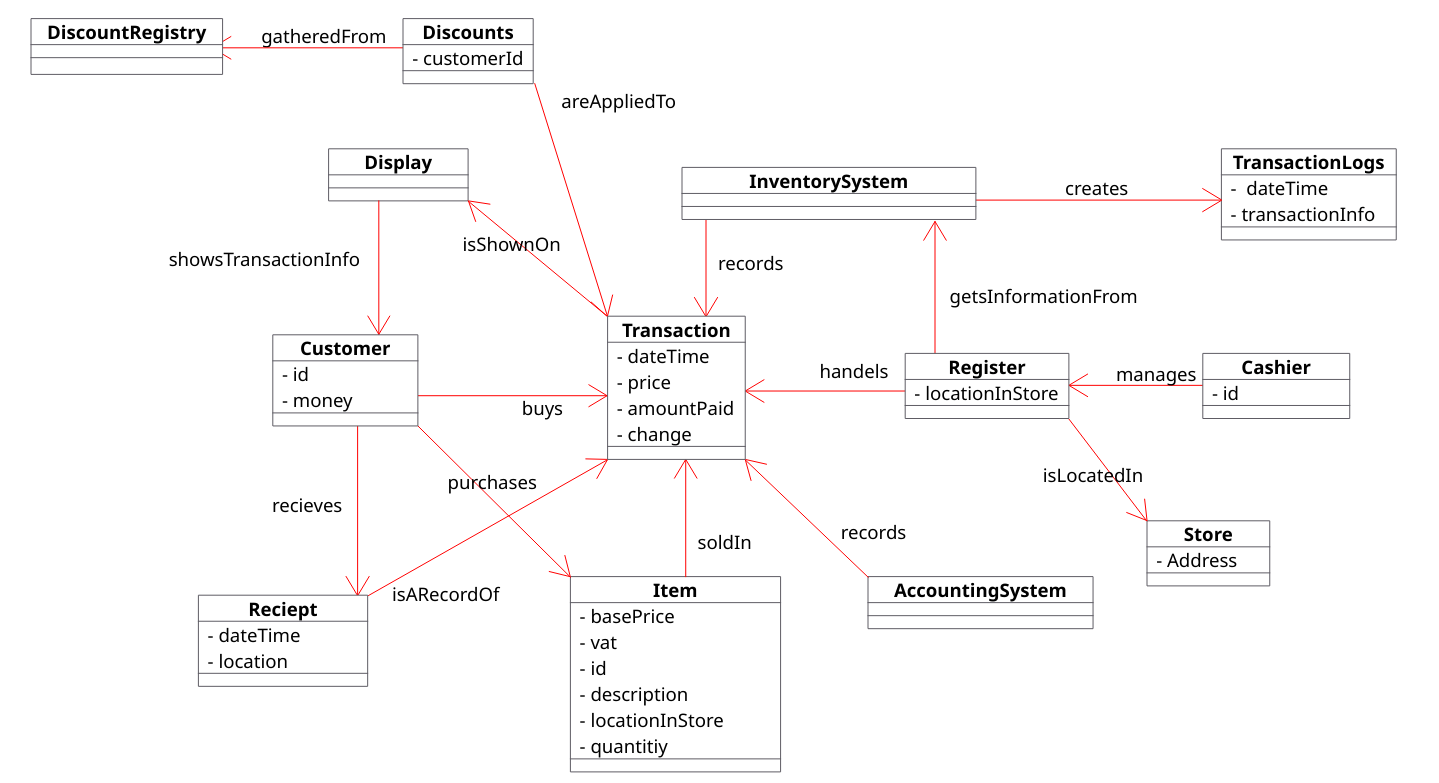
\includegraphics[scale=1.0]{dm1.png}
            \caption{A sample diagram to illustrate caption (this text), numbering and reference in text.}
            \label{fig:dm}
        \end{center}
    \end{figure}

    \begin{figure}[h!]
        \begin{center}
            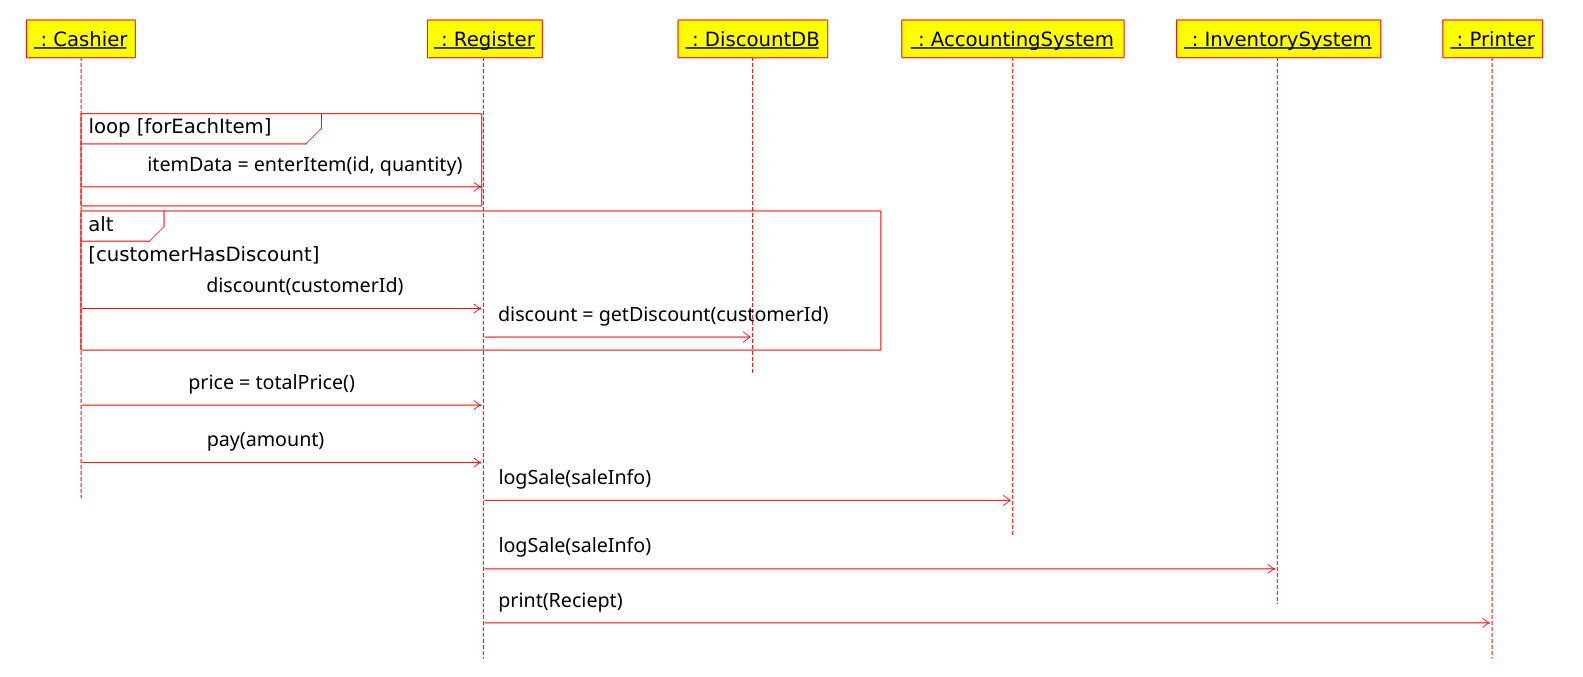
\includegraphics[scale=1.0]{ssd1.png}
            \caption{A sample diagram to illustrate caption (this text), numbering and reference in text.}
            \label{fig:ssd}
        \end{center}
    \end{figure}

\chapter{Discussion}

    % Write an evaluation of the results presented in the result chapter (chapter
    % \ref{sec:result} in this template). To get inspiration for the evaluation,
    % read the assessment criteria in the documents \texttt{assessment-criteria-seminarX.pdf},
    % which are available on the \texttt{Assignments} page of the course web.

    \section{Assesement Criterias}
        \subsection{Typical mistakes are to create a ''programmatic DM'' or a ''naïve DM''. Is the DM either of those?}
            I would not consider the DM naïve since it does not model flow but a
            snapshot of how everything fits together.

        \subsection{ˆAre there ''spider-in-the-web'' classes?}
            I would consider ''Transaction'' to be a bit of a ''spider-in-the-web''.
            However, it is justified because ''Transaction'' is such an essential
            part. Nothing else serves any purpose without a transaction since the
            only point of a store is to facilitate transactions between parties.
            
        \subsection{ˆCan you understand the DM? Is it a correct description of the problem domain?}
            I think that it is clear what the different classes represent and what
            associations they have with other classes. I might be biased though.

        \subsection{ˆDoes the DM have a reasonable number of classes? Are important classes missing?}
            I believe that there's a  number of classes for the given
            requirements, if anything there are too few.

        \subsection{Are there irrelevant classes?}
            Not that I can think of, some classes, like store would probably not
            be useful in a program, but since it's not a program it serves it
            purpose.

        \subsection{ˆDo you agree with the choices between class and attribute?}
            Yes! It might have been better to have another class called 'Payment'
            so that the customer could make a payment and the cashier could
            receive payment, but I do feel that that that would be unnecessary 
            since it wouldn't add any additional information.

        \subsection{ˆIs there a reasonable number of associations? Do you understand them? Are there classes missing associations? If so, is that a mistake?}
            No class is missing associations and I believe the associations are
            clear. More associations could be added, but I don't think that 
            would add any value.

        \subsection{ˆAre naming conventions followed in DM and SSD?}
            The naming conventions follow traditional Java naming conventions.

        \subsection{ˆIs UML used correctly in DM and SSD?}
            Besides the associations having directions I believe the diagramss
            adhere to the UML standard.

        \subsection{ˆAre the correct objects included in the SSD?}


        \subsection{ˆAre the correct operations and return values included in the SSD?}


        \subsection{ˆIs the method and result explained in the report? Is there a discussion? Is the discussion relevant?}

        
\end{document}
